\chapter{Um Passeio pela Bioquímica \label{ap:biomol}}
A bioquímica é a ciência que estuda as formas e funções biológicas em termos químicos. Já no século XVIII, os químicos percebiam a grande diferença entre o mundo inanimado e o mundo vivo: Antoine-Laurent Lavoisier (1743-1794) constatou a relativa simplicidade do ``mundo mineral'' --- não orgânico --- comparada a complexidade dos ``mundos animal e vegetal'' \cite{bioquimicaLehninger}. Ele sabia que esses últimos eram constituídos de moléculas ricas nos elementos carbono, oxigênio, nitrogênio e fósforo, que, devido sua abundância na natureza somada com as suas características químicas, são ótimos para constituírem a complexidade da vida.

\section*{Carbono}
A química dos organismos vivos está organizada em torno do carbono, pois este é muito comum na natureza e possuí uma ótima propriedade estrutural: O carbono pode formar ligações simples estáveis com até quatro outros átomos. De fato, o carbono constitui mais da metade do peso seco das células. 

Sabe-se, através de experimentos de cristalografia \cite{ramachandran1974MolStructure}, muito sobre a geometria das ligações dos átomos de uma proteína. Em particular, as quatro ligações simples do carbono formam um tetraedro (vide Figura ~\ref{fig:carbono}, retirada de \cite{bioquimicaLehninger}) com ângulos de 109,5\textdegree entre duas ligações quaisquer e comprimento médio de ligação de 1,54\AA\footnote[1]{Unidade física para distâncias atômicas é o Ângstron (\AA), onde equivale a 1\AA = $10^{-10}$ m.}. Existe também uma outra característica muito importante para nós nas ligações do carbono: Sabe-se que as ligações simples podem rotacionar livremente (a menos que grupos muito grandes ou altamente carregados estejam ligados aos átomos de carbono, onde, neste caso --- e, na verdade, esse é o caso comum ---, a rotação é regida pelo equilíbrio de forças na molécula \cite{carlileTese}, que pode ser limitada), enquanto que as ligações duplas são mais curtas (em torno de 1,34\AA) e não permitem rotação. Perceba também o plano formado pelos átomos A, B, X e Y na Figura ~\ref{fig:carbono}.

\begin{figure}[H]
	\begin{center}
		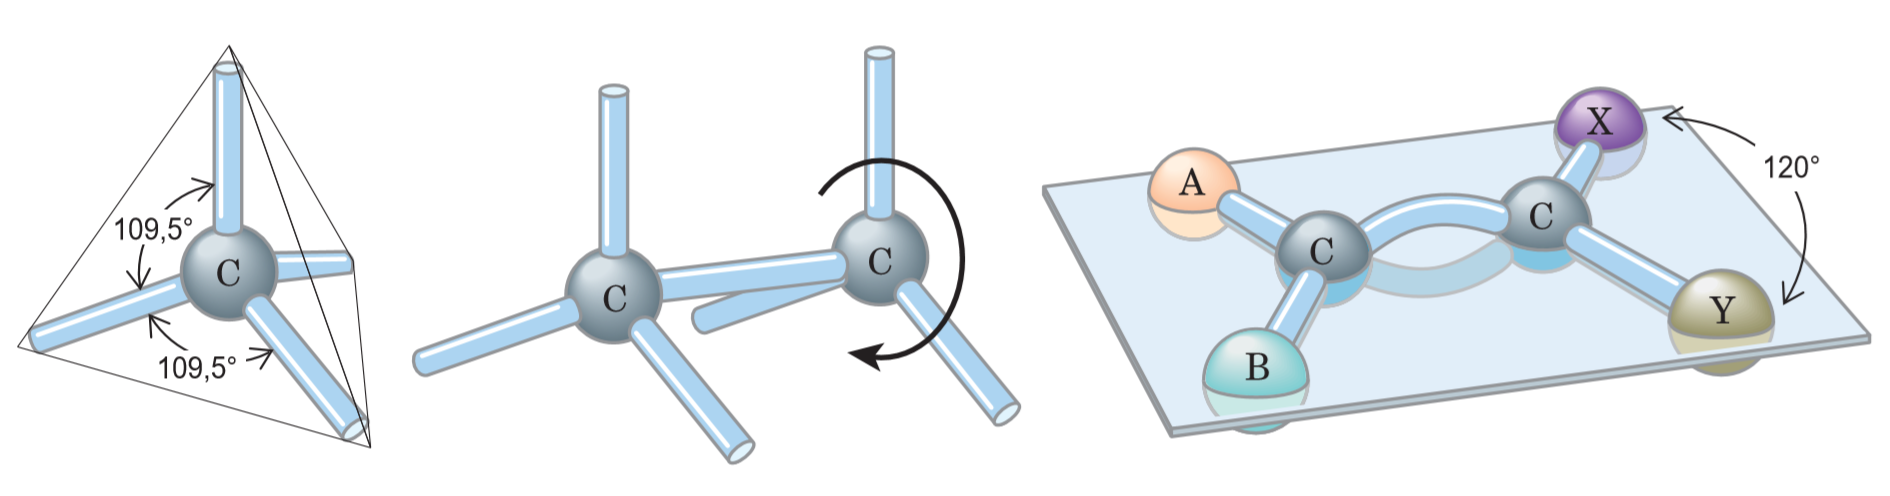
\includegraphics[width=1\linewidth]{secProteins/figures/carbono.png}
	\end{center}
	\caption{Geometria da ligação do carbono.}
	\label{fig:carbono}
\end{figure}

A versatilidade das ligações covalentes do carbono podem formar cadeias lineares, ramificadas e estruturas cíclicas. Nenhum outro elemento químico consegue formar moléculas com tanta diversidade de tamanhos, formas e composição.

\section*{Classificação Macromolecular}
As células contém um conjunto universal de moléculas pequenas. Mas como podemos discutir sobre o que é uma molécula pequena? Devemos definir uma forma de comparar os tamanhos moleculares. Na literatura existem duas medidas principais para esse fim, com uma relação bem definida entre si, tratam-se do \textit{peso molecular} (ou \textit{massa molecular relativa}), denominado $M_r$ e da \textit{massa molecular}, denotada simplesmente por $m$.

O peso molecular é definido como uma relação direta da massa da molécula da substância estudada com um duodécimo da massa do carbono-12 ($^{12}C$, em torno de $1,9926\times 10^{-23}$ gramas), note que, como $M_r$ é uma razão, não possui dimensão associada. Já a massa molecular é apenas a massa da molécula (ou massa molar) sobre o número de Avogadro --- que é definida como sendo o número de átomos por mol de uma determinada substância. Esta, diferente da massa molecular relativa, possui dimensão e é expressa em dáltons (abreviado Da) e um dálton equivale a um duodécimo da massa do carbono-12 --- donde deduze-se facilmente a relação entre massa molecular e peso molecular.

Os organismos vivos são constituídos por moléculas de características muito diversas. Existe uma coleção de aproximadamente mil moléculas consideradas pequenas ($M_r$ ${\sim}100$ a ${\sim}500$) diferentes dissolvidas na fase aquosa das células \cite{bioquimicaLehninger}. Nessa coleção está contido os aminoácidos comuns, nucleotídeos, açúcares e seus derivados fosforilados e ácidos mono, di e tricarboxílicos. Porém, neste estudo, estaremos mais preocupados com moléculas significativamente maiores, chamadas \textit{macromoléculas}.
\subsection*{Macromoléculas}
As macromoléculas são as principais constituintes das células. São polímeros\footnote[1]{Polímeros são moléculas formadas a partir de repetições de unidades estruturais menores, chamadas \textit{meros} ou \textit{monômeros}. Daí o nome, poli-meros $\approx$ vários-meros.} com peso molecular acima de ${\sim}5.000$. Polímeros menores são chamados de \textit{oligômeros} --- do grego, ``oligos'' significa ``pouco''. Proteínas (principal molécula do nosso estudo), ácidos nucleicos (DNA, RNA) e polissacarídeos são macromoléculas feitas de monômeros cujos pesos moleculares são de 500 ou menos, porém, como apresentam um grande número dessas subunidades, possuem um alto peso molecular --- até 1 milhão para proteínas e até vários bilhões para ácidos nucleicos. A síntese de macromoléculas é a atividade mais custosa energeticamente das células.

Tanto as proteínas quanto os ácidos nucleicos são polímeros lineares (isto é, que não possuem ramos ligados as suas cadeias principais, agindo como um longo fio contínuo) feitos de subunidades monoméricas bem mais simples, donde esta sequência específica de meros é que dá as informações sobre a sua estrutura tridimensional e suas funções biológicas associadas \cite{bioquimicaLehninger}.

Em especial, as proteínas são constituídas por um conjunto de monômeros muito bem conhecidos e catalogados, chamados \textit{aminoácidos}. As proteínas constituem a segunda maior fração da célula, só perdendo para a água. Provavelmente são as mais versáteis de todas as biomoléculas: Algumas tem atividade catalítica e funcionam como enzimas, outras servem como elementos estruturais, receptoras de sinais, ou transportadoras que carregam substâncias específicas para dentro ou fora das células.  

\section*{Configuração Molecular}
No mundo biomolecular, toda a informação sobre uma molécula é dada pela sua estrutura (também chamada de \textit{estereoquímica}), logo, suas ligações covalentes e seus grupos funcionais (subestruturas padrões associadas) são trivialmente importantes para definir seu bom funcionamento. Devido a característica rotacional das ligações simples do carbono, existem muitas moléculas (chamadas \textit{estereoisômeros}) com a mesma fórmula molecular e ligações químicas, mas com diferentes configurações espaciais, o que pode mudar completamente suas funções. 

De maneira simples, podemos identificar estereoisômeros pelo fato de que eles possuem as mesmas propriedades químicas, porém, não podem ser convertidos entre si sem que haja a quebra de uma ou mais ligações covalentes. Isto se dá pela presença de ligações duplas (devido a limitação na sua rotação) ou pela presença de \textit{centros quirais}, onde a molécula rotacionada não pode corresponder a sua imagem especular (conforme Figura ~\ref{fig:quiral}, extraída de \cite{bioquimicaLehninger}). Um átomo de carbono com quatro ligações diferentes é considerado assimétrico e é chamado de centro quiral --- do grego, \textit{chiros} quer dizer "mão", parafraseando estas estruturas com a relação da mão direita com a esquerda. Logo, se existir um centro quiral, sempre haverá pelo menos duas possibilidades para configuração.

\begin{figure}[H]
	\begin{center}
		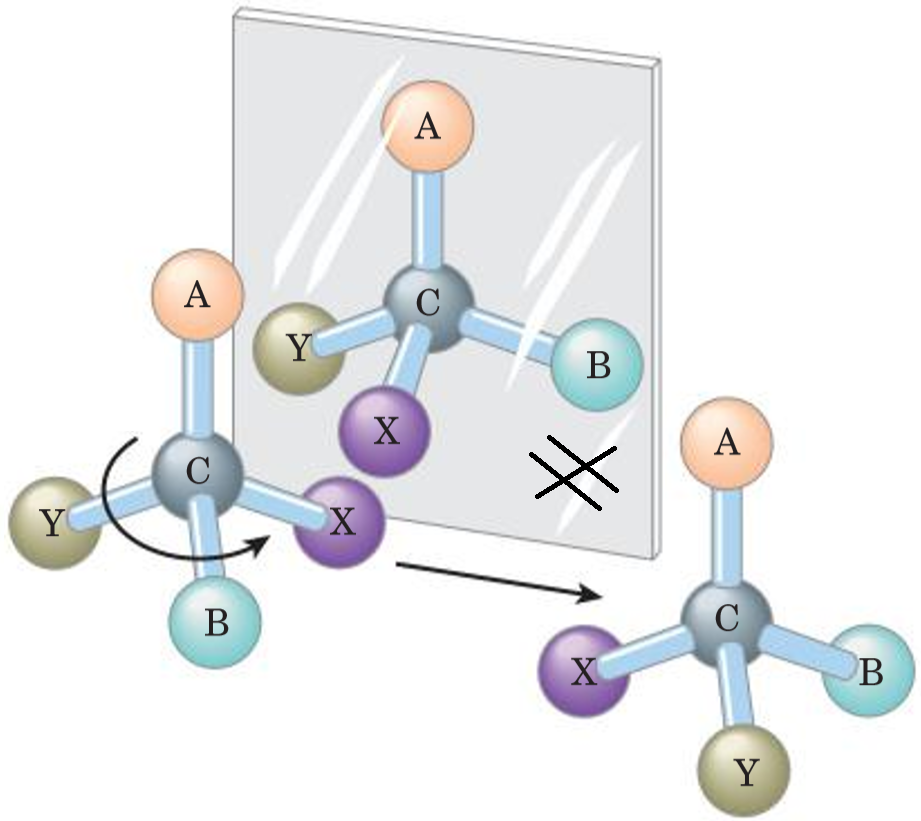
\includegraphics[width=0.45\linewidth]{secProteins/figures/quiral.png}
	\end{center}
	\caption{Ilustração de uma molécula quiral.}
	\label{fig:quiral}
\end{figure} 

Outro conceito que nos será importante no futuro, a \textit{conformação molecular} é a disposição dos átomos no espaço que pode ser mudada por rotação em torno de ligações simples, sem quebrar ligações covalentes. Estes ângulos possíveis tem posições mais estáveis e instáveis do ponto de vista energético, conforme mostra o gráfico da Figura ~\ref{fig:carener}. Podemos tentar descobrir a conformação mais provável de uma molécula minimizando a somatória de todas as forças atuantes na molécula \cite{carlileTese}. 

\begin{figure}[H]
	\begin{center}
		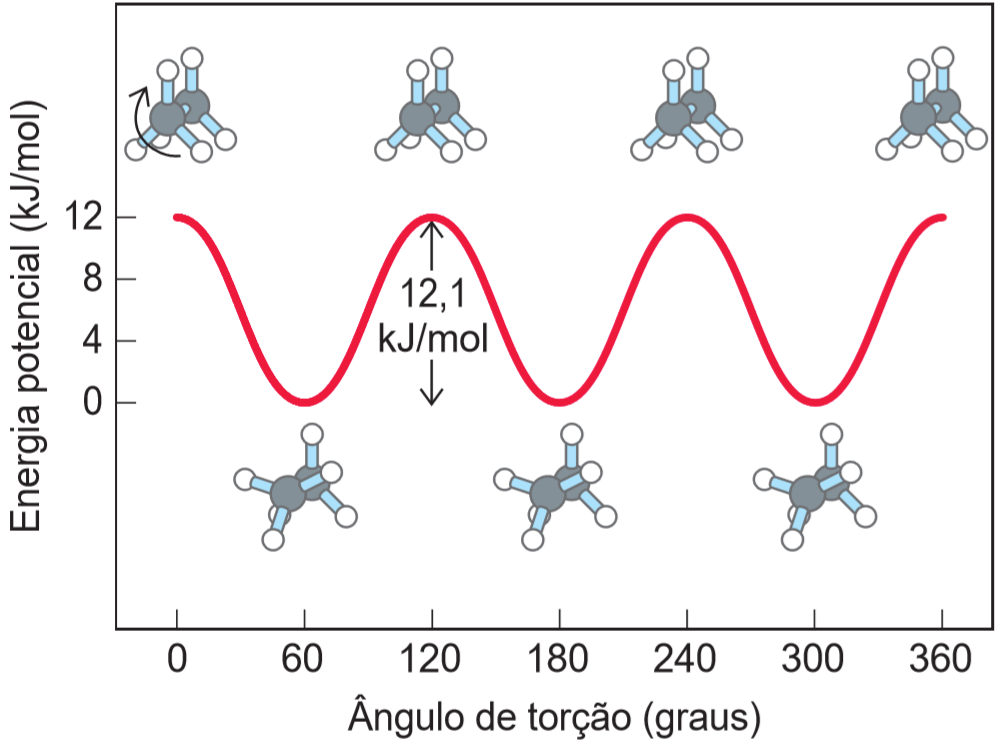
\includegraphics[width=0.55\linewidth]{secProteins/figures/carbonoenergia.png}
	\end{center}
	\caption{Conformações e Equilíbrio de Energia \cite{bioquimicaLehninger}.}
	\label{fig:carener}
\end{figure} 

Para compreender melhor como serão as configurações das moléculas que trataremos nesse texto (proteínas), vale nos preocuparmos com as subestruturas do qual eles são formados. 

\section*{Aminoácidos}
As proteínas são longas cadeias lineares de aminoácidos ligados por um tipo específico de ligação (chamada \textit{peptídica}), a qual é característica por ter como resíduo uma molécula de água. São vinte tipos diferentes de aminoácidos encontrados normalmente na natureza, sendo esses muito bem conhecidos e catalogados. O primeiro a ser descoberto foi a asparagina, em 1806; o ultimo foi a treonina, descoberto em 1938 \cite{bioquimicaLehninger}. Vale mencionar que, além destes vinte aminoácidos mais comuns, há vários outros menos frequentes, porém não constituem as proteínas.

Destes vinte aminoácidos comuns (disponíveis no Apêndice C), dezenove compartilham da mesma estrutura principal \cite{fidalgotese} --- estes são chamados $\alpha$-aminoácidos. Eles tem um grupo carboxílico e um grupo amina ligados ao mesmo átomo de carbono (o carbono $\alpha$), além de mais um hidrogênio (chamado hidrogênio $\alpha$) e, em sua última ligação, uma cadeia R que é o que diferencia cada aminoácido. Essa estrutura é ilustrada na Figura ~\ref{fig:amino}. O único aminoácido que difere disso é a Prolina, que possui como cadeia R um anel aromático que se fecha no nitrogênio (que no padrão mencionado há um grupo amina).

\begin{figure}[H]
	\begin{center}
		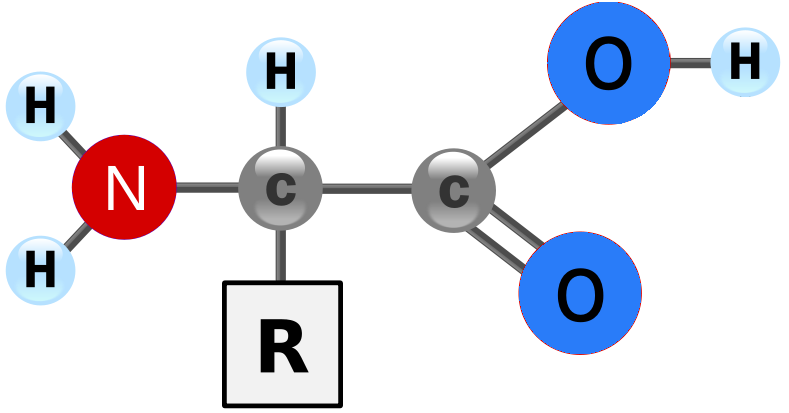
\includegraphics[width=0.35\linewidth]{secProteins/figures/amino.png}
	\end{center}
	\caption{Estrutura padrão de um $\alpha$-aminoácido.}
	\label{fig:amino}
\end{figure}

Portanto, há uma noção prévia de qual tipo de estrutura esperar ao analisar uma molécula de proteína. Existe uma estrutura conhecida e repetitiva para os átomos.

Para todos os aminoácidos comuns, exceto a glicina, o carbono $\alpha$ está ligado com quatro outros átomos diferentes entre si (na glicina temos R como apenas mais um hidrogênio, sendo o aminoácido mais simples), o que transforma o carbono $\alpha$ em um centro quiral. Logo, cada aminoácido (menos glicina) tem sempre dois estereoisômeros possíveis. Porém, na verdade, apenas um destes ocorrê naturalmente nas proteínas \cite{bioquimicaLehninger}.

\subsection*{Ligação Peptídica}
A ligação entre dois aminoácidos é feita de modo covalente por meio de desidratação do grupo $\alpha$-carboxílico de um com o grupo $\alpha$-amina do outro --- ou seja, ligar o carbono final de um no nitrogênio inicial do outro, liberando um oxigênio e dois hidrogênios, que formam uma molécula de água. Essa ligação, também chamada de resíduo (devido a liberação da água), forma um dipeptídeo. 

Quando muitos aminoácidos se juntam, o produto é chamado de polipeptídeo. Perceba que os termos ``polipeptídeo'' e ``proteína'' parecem dirigir-se as mesmas moléculas, porém, a diferença está na massa molecular: As moléculas com massa abaixo de 10.000 são ditas polipeptídeos, enquanto as maiores que essas são consideradas proteínas. Os comprimentos dessas cadeias variam significativamente. O citocromo c humano tem apenas 104 aminoácidos, enquanto, no outro extremo, a titina (relacionada ao músculo de vertebrados) possui aproximadamente 27.000 aminoácidos e uma massa molecular de cerca de 3.000.000. No geral, as proteínas naturais contém menos de 2.000 aminoácidos \cite{bioquimicaLehninger}.

Outra característica muito importante das ligações peptídicas é de que elas se comportam semelhantemente a ligações covalentes duplas dos carbonos. Estudos envolvendo difração de raios X em cristais de aminoácidos e polipeptídeos descobriram que a ligação peptídica $C-N$ é de alguma forma mais curta que a ligação de uma amina simples, e que os átomos associados a ligação peptídica estão todos co-planares (conforme Figura ~\ref{fig:peptidica}). Perceba que também são rígidos, não sendo possível a rotação. Essa é uma propriedade muito útil que também nos será importante, descoberta de 1930 que se deve a Linus Pauling e Robert Corey.

\begin{figure}[H]
	\begin{center}
		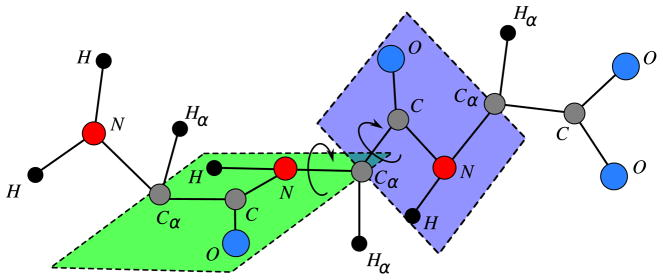
\includegraphics[width=0.8\linewidth]{secProteins/figures/peptide.jpg}
	\end{center}
	\caption{O grupo peptídico planar \cite{carlile:MinimalOrder}.}
	\label{fig:peptidica}
\end{figure}

\section*{Estrutura das Proteínas}
A estrutura de proteínas pode ser descrita em quatro níveis de importante hierarquia conceitual, conforme pode ser visto na Figura ~\ref{fig:protest}, retirado de \cite{bioquimicaLehninger}. A estrutura primaria consiste da mais detalhada, sendo de fato os polímeros de aminoácidos; Estes, por sua vez, formam alguns arranjos particularmente estáveis, que dão origem a padrões estruturais recorrentes, que chamamos de \textit{estruturas secundárias} (como as hélices $\alpha$, as duplas hélices etc..). A estrutura terciária descreve todos os aspectos do enovelamento tridimensional de um polipeptídeo, ou seja, define quais serão as forças atuantes na molécula --- que da origem a sua conformação estável, que minimiza a energia livre de Gibbs do sistema. Quando existem mais estruturas terciárias em uma proteína, chamamos a junção destas de estrutura quaternária.	

\begin{figure}[H]
	\begin{center}
		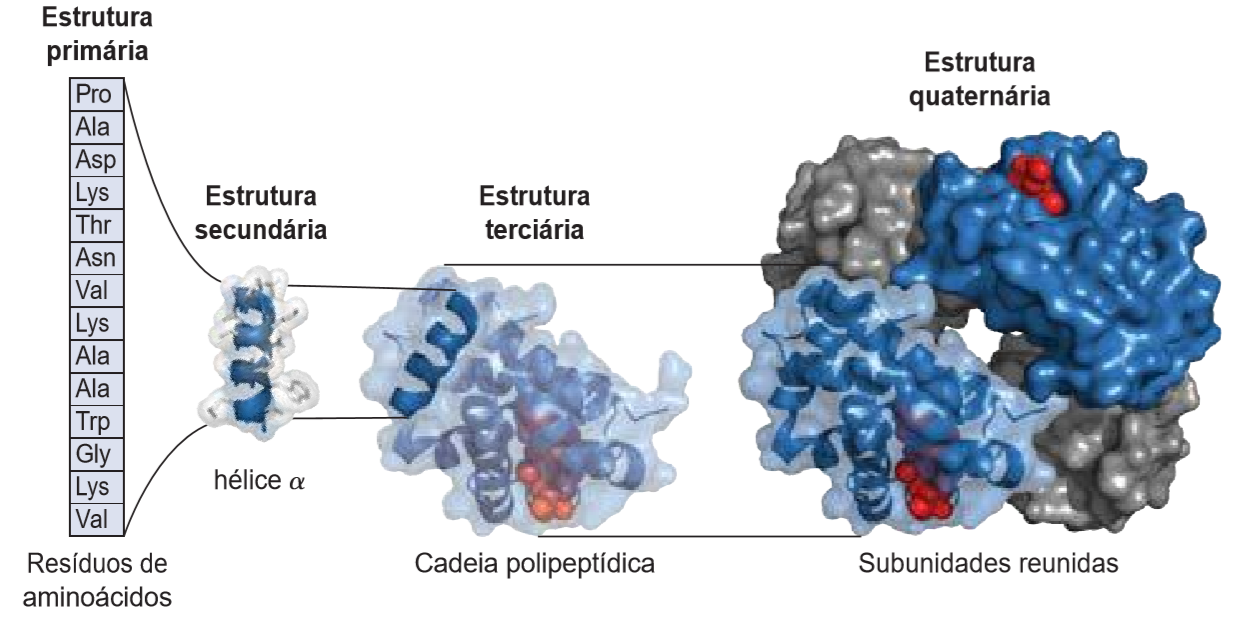
\includegraphics[width=0.9\linewidth]{secProteins/figures/protest.png}
	\end{center}
	\caption{Níveis de estrutura das proteínas exemplificados na Hemoglobina.}
	\label{fig:protest}
\end{figure}

Em especial, as diferentes configurações da estrutura primária --- que pode mudar drasticamente entre estruturas primárias diferentes na mesma molécula --- nos é mais informativa. A estrutura primária de uma proteína determina como ela se dobra em sua estrutura tridimensional, devido os ângulos e distâncias bem definidos de suas ligações entre átomos, que da a sua estrutura especial; o que, por sua vez, determina a função da proteína --- como no exemplo da Figura ~\ref{fig:protest}, onde a estrutura da hemoglobina é que permite que átomos de oxigênio ``encaixem'' nela, possibilitando o transporte desse átomo pelo organismo, que é sua função (e só o é dado sua estrutura tridimensional). 

Por sua relação com a estrutura tridimensional e, logo, função das proteínas, vamos nos concentrar em estudar a subdivisão de estruturas primárias. 

\subsection*{A Cadeia Principal de uma Proteína}
Quando se estuda proteínas a nível dos aminoácidos, não tardamos a perceber que elas possuem uma estrutura repetida muito interessante do ponto de vista bioquímico. Trata-se da \textit{cadeia principal} de uma proteína, também chamada de \textit{Backbone} --- espinha dorsal, em tradução literal, fazendo alusão a importância desta estrutura. Perceba que os vinte aminoácidos que compõem as proteínas possuem sempre os mesmos três átomos ligados em sequência (Figura ~\ref{fig:backbone}): $N-C_\alpha-C$, através de ligações covalentes em torno do $C_\alpha$ e da ligação peptídica $C-N$ entre aminoácidos.

\begin{figure}[H]
	\begin{center}
		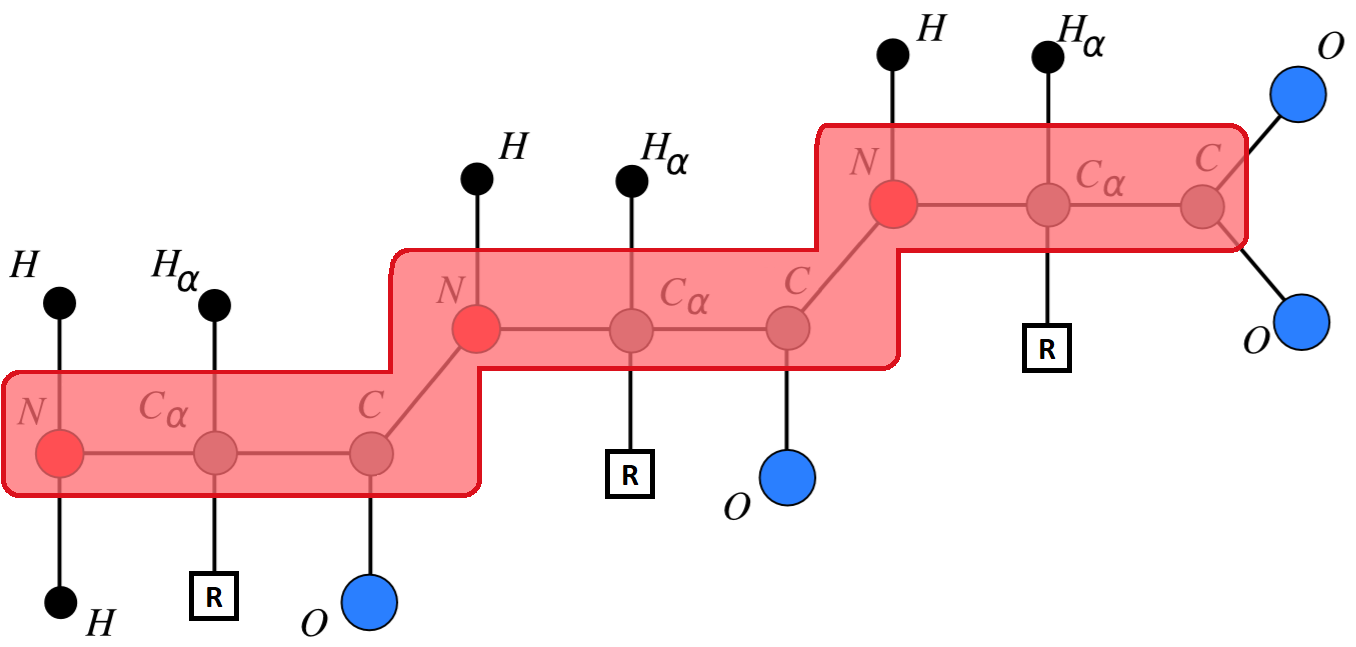
\includegraphics[width=0.8\linewidth]{secProteins/figures/backbone.png}
	\end{center}
	\caption{Representação da cadeia principal da proteína, adaptada de  \cite{carlile:MinimalOrder}}.
	\label{fig:backbone}
\end{figure}

Outra informação bastante útil sobre esta cadeia principal é que, devido dados experimentais de cristalografia, sabe-se sobre a geometria média dessa subestrutura \cite{ramachandran1974MolStructure}, onde os comprimentos e ângulos entre  as ligações dos átomos que a formam são fixas, na média, a menos de erros de medida. Vide Figura ~\ref{fig:rama}, extraída do texto original de Ramachandran \textit{et al}, um dos precursores deste estudo.

\begin{figure}[H]
	\begin{center}
		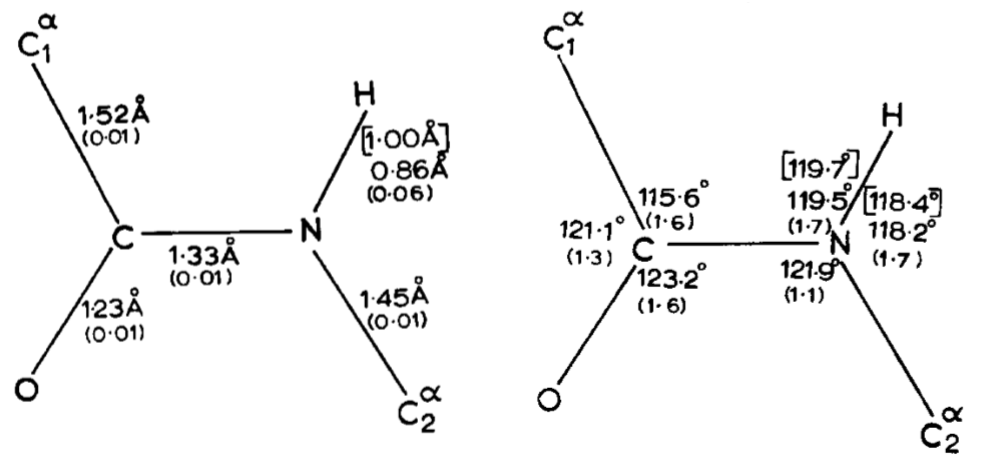
\includegraphics[width=0.8\linewidth]{secProteins/figures/rama.png}
	\end{center}
	\caption{Dados de ângulos e distâncias médios de ligações em um aminoácido.}
	\label{fig:rama}
\end{figure}


\section*{\textit{Worldwide Protein Data Bank}}
Já foi possível perceber a grande variedade de diferentes configurações possíveis para as proteínas. Com isso, há a necessidade de se estudar cada uma explicitamente, através de experimentos, catalogando e guardando essas informações. Esse grande esforço para entender o mundo das macromoléculas se deixa transparecer com o repositório \textit{Worldwide Protein Data Bank} --- ou simplesmente wwPDB \cite{wwPDB}.

Este é um repositório online e público onde estão guardadas todas os dados de proteínas e ácidos nucleicos já catalogados, em especial dados de suas estruturas 3D (posições x, y e z de cada um dos átomos que a constituem). Auxiliando tanto pesquisadores, quanto professores e estudantes, essa base de dados é um grande esforço em conjunto de físicos, biólogos, bioquímicos e vários outros profissionais de diversas áreas do conhecimento de todo o mundo.

\subsection*{Arquivo PDB}
Quando se quer estudar uma proteína no repositório PDB, base fazer o \textit{download} do arquivo PDB da molécula (extensão ``.ent''). Esse é um arquivo de estruturas tridimensionais de macromoléculas biológicas determinadas experimentalmente, que descrevem as coordenadas espaciais de cada átomo cuja posição foi determinada (muitas das estruturas catalogadas não estão completas); também existem dados adicionais sobre informações de como as estruturas foram determinadas, os dados práticos dos experimentos, a precisão associada aos dados e tudo mais que quem estiver criando o documento achar necessário para aquela macromolécula.

Tecnicamente, o arquivo PDB trata-se de uma representação estruturada dos dados moleculares e experimentais da proteína. Ele é separado por seções, onde cada seção pode possuir subseções. São elas: 
\begin{itemize}
	\item \textbf{Seção Title} - Contem a descrição da molécula;
	\vspace{-0.3cm}
	
	\item \textbf{Seção Remark} - Vários comentários sobre anotações de entrada com mais profundidade que os registros padrões;
	\vspace{-0.3cm}
	
	\item \textbf{Seção Primary structure} - Sequências peptídicas ou nucleotídicas especificadas para serem posteriormente utilizadas, diminuindo a repetição do arquivo;
	
	\vspace{-0.3cm}
	\item \textbf{Seção Heterogen} - Descrição de grupos presentes não padronizados --- Visto que proteínas também podem conter materiais inorgânicos, como o ferro presente na hemoglobina (vide Figura ~\ref{fig:protest});
	\vspace{-0.3cm}
	
	\item \textbf{Seção Secondary structure} - Descrição das estruturas secundárias presentes na molécula;
	
	\vspace{-0.3cm}
	\item \textbf{Seção Connectivity annotation} - Descrição das conectividade químicas da molécula;
	\vspace{-0.3cm}
	
	\item \textbf{Seção Miscellaneous features} - Descrição dos recursos dentro da macromolécula;
	\vspace{-0.3cm}
	
	\item \textbf{Seção Crystallographic} - Descrição de parâmetros da cristalografia, quando o experimento utiliza esta metodologia;
	
	\vspace{-0.3cm}
	\item \textbf{Seção Coordinate transformation} - Matrizes como operadores de transformação das coordenadas;
	\vspace{-0.3cm}
	
	\item \textbf{Seção Coordinate} - Dados de coordenadas atômicas, a seção que mais vamos utilizar;
	\vspace{-0.3cm}
	
	\item \textbf{Seção Connectivity} - Citação das conexões químicas entre os átomos;
	\vspace{-0.3cm}
	
	\item \textbf{Seção Bookkeeping} - Resumo das características totais do arquivo e o marcador de fim de arquivo.
\end{itemize}

Como o arquivo é significativamente extenso, não entraremos em detalhes neste texto sobre as características detalhadas de cada uma das seções apresentadas. Porém, vale mencionar o tipo de entrada ATOM, presente na seção Coordinate, pois essa é a entrada que compõe a maior parte dos arquivos PDB, além de ser a de nosso interesse principal.

A entrada ATOM tem como objetivo descrever detalhes de cada átomo específico da molécula. Ela segue um padrão indentado, onde cada dado é caracterizado pela sua posição na linha (coluna). Segue principais dados da entrada e suas respectivas colunas na Tabela ~\ref{table:atom}.

\begin{table}[h!]
	\centering
	\begin{tabular}{ |c|c| } 
		\hline
		Código serial do átomo & 7-11 \\ 
		\hline
		Nome do átomo & 13-16 \\ 
		\hline
		Nome do resíduo que pertence & 18-20 \\ 
		\hline
		Identificador da cadeia & 22 \\ 
		\hline
		Código serial de dentro do resíduo & 23-26 \\ 
		\hline
		Coordenada x & 31-38 \\ 
		\hline
		Coordenada y & 39-46 \\ 
		\hline
		Coordenada z & 47-54 \\ 
		\hline
		\textit{Occupancy} do átomo & 55-60 \\ 
		\hline
		Fator de temperatura & 61-66 \\ 
		\hline
		Simbolo do elemento & 77-78 \\
		\hline
	\end{tabular}
	\caption{Principais dados da entrada ATOM.}
	\label{table:atom}
\end{table}

\vspace{-0.4cm}
Segue exemplo de um conjunto de entradas do tipo ATOM na Figura ~\ref{fig:atom}.
\begin{figure}[H]
	\begin{center}
		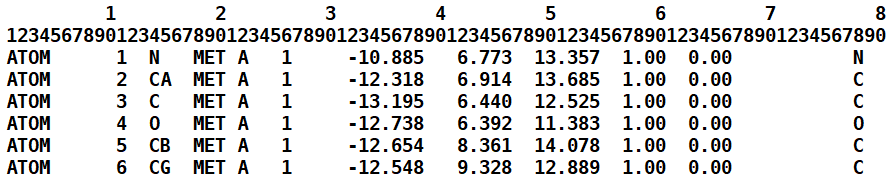
\includegraphics[width=0.95\linewidth]{secProteins/figures/atom.png}
	\end{center}
	\caption{Conjunto de entradas do tipo ATOM.}
	\label{fig:atom}
\end{figure}
\vspace{-0.3cm}

Com esse conjunto de dados, pode-se, por exemplo, esboçar uma representação gráfica de uma molécula. Existem muitos softwares compatíveis com os arquivos PDB para este fim, por exemplo, o autor deste documento implementou uma visualização de uma projeção da molécula 3D no plano z = 0, como pode-se averiguar na Figura~\ref{fig:molproj}.

\begin{figure}[H]
	\begin{center}
		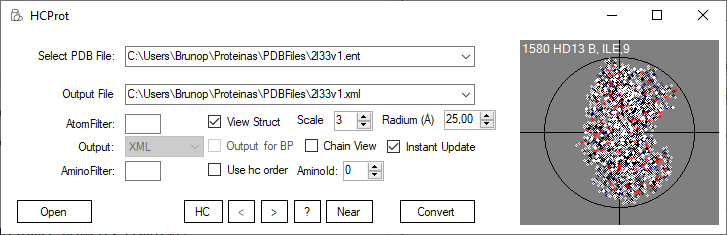
\includegraphics[width=1\linewidth]{secProteins/figures/molproj.png}
	\end{center}
	\caption{HCProt com visualização a partir de um aquivo PDB.}
	\label{fig:molproj}
\end{figure}


Aqui vale um momento para uma introdução ao software desenvolvido, como parte dos resultados deste trabalho. 
\subsection*{\textit{Sotware HCProt}}
O arquivo PDB é denso, cheio de termos técnicos e pouco amigável, demandando um certo tempo para que alguém que esteja sendo introduzido nesta área se acostume com seu padrão. Por isso, surgiu a possibilidade de desenvolver uma aplicação que vise facilitar e automatizar a extração das informações das moléculas contidas nele. Este trabalho teve esse software, nomeado \textit{Protein Data Bank Reader}, como primeiro resultado prático.

O software foi desenvolvido em C${^\#}$, uma linguagem de programação multiparadigma, orientada a objetos e eventos, de tipagem forte, desenvolvida pela Microsoft como parte do \textit{framework }.NET. A interface de usuário foi feita utilizando Windows Forms, como uma janela única, denominada fMain (que pode ser vista na Figura ~\ref{fig:molproj}).

A aplicação pode ser usada de duas formas diferentes: Para gerar um arquivo bem formatado com os dados dos átomos contidos no arquivo PDB de entrada --- isso pode ser feito em diversos formatos, como XML, JSON, Matriz (no padrão MatLAb) e MolConf (padrão para aplicar na biblioteca Julia Language MolecularConformation.jl \cite{emersonMolConf}); Ou pode ser usado apenas como ferramenta de visualização da molécula (selecionando o \textit{checkbox} struct view).

\begin{figure}[H]
	\begin{center}
		%\hspace{-1cm}
		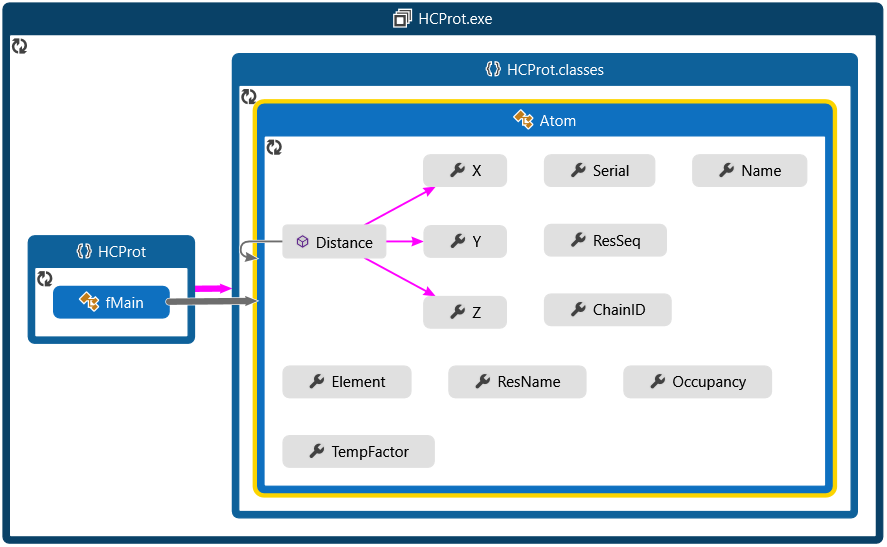
\includegraphics[width=0.95\linewidth]{secProteins/figures/classDiagram.png}
	\end{center}
	\caption{Relação entre classes do HCProt.}
	\label{fig:classDiagram}
\end{figure}

Observe na Figura ~\ref{fig:classDiagram} a existência de um conjunto de classes em \textit{HCProt.class} que o formulário fMain utiliza. Em especial, a classe Atom, que representa um átomo, contendo todos as suas propriedades (retiradas do arquivo PDB, como as posições x, y e z) e uma função muito importante, chamada \textit{Distance}, que retorna a distância euclidiana entre dois átomos.

O formulário fMain possui um conjunto de eventos, disparados por interações com o usuário (como mostrado na Figura ~\ref{fig:fmain}). Como pode-se perceber pelo diagrama, a grande maioria dos eventos chamam o método \textit{updateView}, que tem a função de atualizar a tela de visualização da proteína. Perceba que isso só acontece quando se está com o checkbox \textit{structView} selecionado, uma vez que o updateView só funciona nesse caso.

\begin{figure}[H]
	\begin{center}
		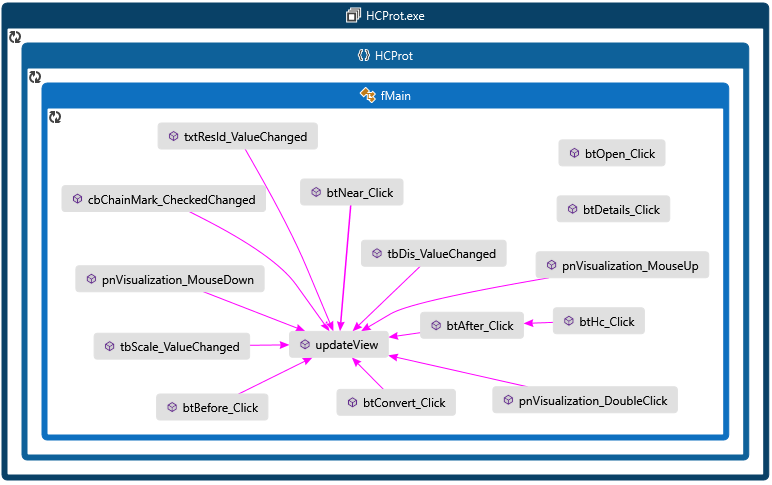
\includegraphics[width=0.95\linewidth]{secProteins/figures/fmainClassDiagram.png}
	\end{center}
	\caption{Respostas do formulário ás ações do usuário.}
	\label{fig:fmain}
\end{figure}

\subsection*{Definição das funções do HCProt}
Segue abaixo uma descrição dos principais componentes do software que permitem interação com o usuário. Verifique a presença dos identificador \textit{id} de cada componente na Figura ~\ref{fig:HCProt}, que são referenciados na Tabela ~\ref{table:HCProt} com suas respectivas descrições.

\begin{figure}[H]
	\begin{center}
		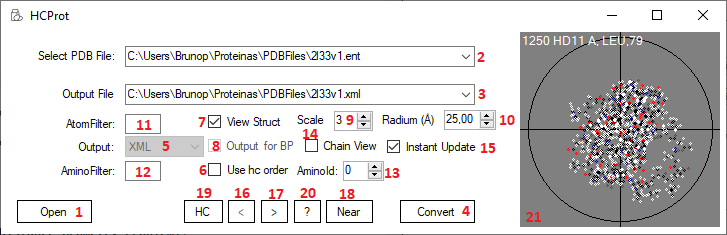
\includegraphics[width=1\linewidth]{secProteins/figures/HCProt.png}
	\end{center}
	\caption{Interação do HCProt.}
	\label{fig:HCProt}
\end{figure}

\begin{table}[H]
	\hspace{-2cm}
	%\centering
	\begin{tabular}{ |c|c|c| } 
		\hline
		\textbf{id} & \textbf{Tipo} & \textbf{Descrição} \\
		\hline
		1 & Botão & Abre uma caixa de diálogo para selecionar o arquivo PDB de entrada \\\hline
		2 & Caixa de Texto & Diretório onde está o arquivo de entrada \\ \hline
		3 & Caixa de Texto & Diretório para onde será gerado o arquivo de saída\\\hline
		4 & Botão & Realiza a leitura do arquivo e faz a conversão\\\hline
		5 & Combo de Seleção & Seleciona o formato do arquivo de saída \\\hline
		6 & Caixa de Seleção & Seleciona se é para usar o Ordenação HC durante a conversão \\ \hline
		7 & Caixa de Seleção & Seleciona se o objetivo é ter uma visualização da molécula\\ \hline
		8 & Caixa de Seleção & Seleciona se será usado o padrão Branch-and-Prune na conversão\\ \hline
		9 & Entrada Numérica & Informa qual a escala para ser usada na visualização\\ \hline
		10 & Entrada Numérica & Informa o raio a ser considerado na conversão e visualização\\ \hline
		11 & Caixa de Texto & Filtrar por algum átomo específico (e.g. ``C'' para carbono)\\ \hline
		12 & Caixa de Texto & Filtrar por algum aminoácido específico (e.g. ``ALA'' para Alanina)\\ \hline
		13 & Entrada Numérica & Se > 0 filtra para o aminoácido de identificador específico\\ \hline
		14 & Caixa de Seleção & Se selecionado pinta de rosa todas as cadeias que não forem a primeira\\ \hline
		15 & Caixa de Seleção & Se deseja que o software atualize o painel sempre que houver alterações.\\ \hline
		16 & Botão & Permite movimentação entre átomos, centraliza a tela no átomo anterior\\ \hline
		17 & Botão & Permite movimentação entre átomos, centraliza a tela próximo átomo\\ \hline
		18 & Botão & Centraliza o painel no átomo com menor distância para o atual\\ \hline
		19 & Botão & Tenta percorrer o aminoácido atual usando a ordem HC de forma empírica\\ \hline
		20 & Botão & Abre uma janela com informações sobre o átomo atual e os próximos\\ \hline
		21 & Painel Visual & Centraliza o painel em um átomo clicando duas vezes nele\\\hline
	\end{tabular}
	\caption{Descrição dos componentes do software.}
	\label{table:HCProt}
\end{table}

Por exemplo, pode-se estudar apenas o segundo aminoácido (Alanina) da proteína Calcyclin (codigo PDB 1A03) --- uma proteína do tipo ligante de cálcio --- apenas setando o AminoId (componente 13 da Figura ~\ref{fig:HCProt}) para 2 e selecionando o View Sctruct (componente 7). Também podemos alterar a escala de exibição (componente 9) e a distância radial de visão (componente 10), para facilitar a visualização nessa dimensão pequenina. O resultado se vê na Figura ~\ref{fig:exemploView}.

\begin{figure}[H]
	\hspace{-1.3cm}
	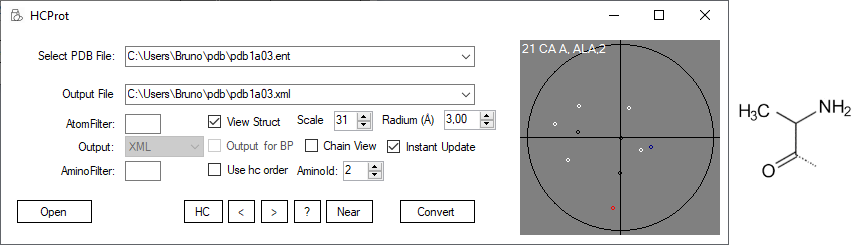
\includegraphics[width=1.2\linewidth]{secProteins/figures/exemploView.png}
	\caption{Visualização de uma Alanina utilizando o HCProt.}
	\label{fig:exemploView}
\end{figure}

\chapter{Vinte Aminoácidos Naturais} 

É comum dividirmos os aminoácidos proteicos em cinco classes, como segue.
\subsubsection*{Grupos R apolares, alifáticos}
\begin{figure}[H]
	\begin{center}
		\begin{minipage}{0.24\linewidth}
			\centering   
			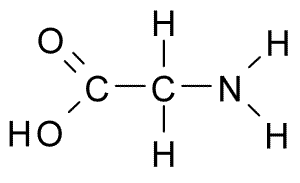
\includegraphics[width=0.95\linewidth]{secProteins/figures/glycine.png}	
			\caption{Glicina}
			\label{fig:glycine}
		\end{minipage}
		\begin{minipage}{0.24\linewidth}
			\centering   
			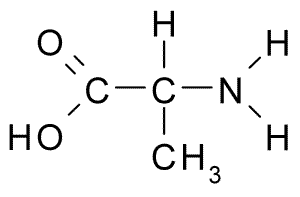
\includegraphics[width=0.9\linewidth]{secProteins/figures/alanine.png}
			\caption{Alanina}
			\label{fig:alanine}
		\end{minipage}
		\begin{minipage}{0.24\linewidth}
			\centering   
			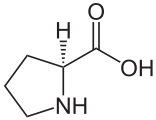
\includegraphics[width=0.8\linewidth]{secProteins/figures/proline.png}
			\caption{Prolina}
			\label{fig:proline}
		\end{minipage}
		\begin{minipage}{0.24\linewidth}
			\centering   
			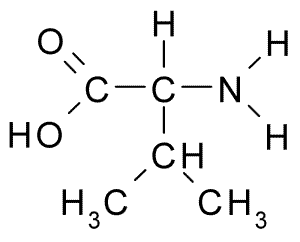
\includegraphics[width=0.8\linewidth]{secProteins/figures/valine.png}
			\caption{Valina}
			\label{fig:valine}
		\end{minipage}
	\end{center}
\end{figure}
\vspace{-1cm}
\begin{figure}[H]
	\begin{center}
		\begin{minipage}{0.3\linewidth}
			\centering   
			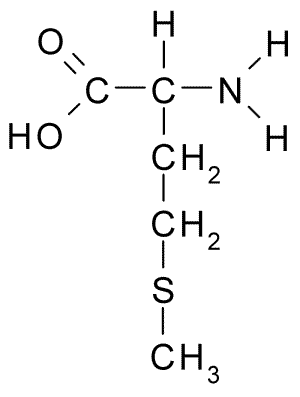
\includegraphics[width=0.63\linewidth]{secProteins/figures/methionine.png}	
			\caption{Metionina}
			\label{fig:methionine}
		\end{minipage}
		\begin{minipage}{0.3\linewidth}
			\centering   
			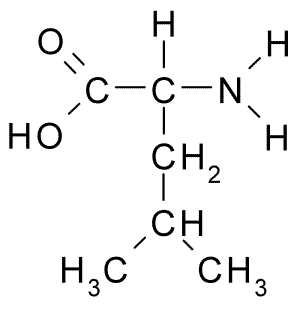
\includegraphics[width=0.8\linewidth]{secProteins/figures/leucine.png}
			\caption{Leucina}
			\label{fig:leucine}
		\end{minipage}
		\begin{minipage}{0.3\linewidth}
			\centering   
			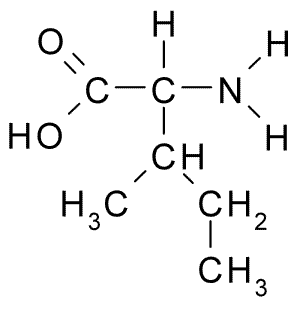
\includegraphics[width=0.8\linewidth]{secProteins/figures/isoleucine.png}
			\caption{Isoleucina}
			\label{fig:isoleucine}
		\end{minipage}
	\end{center}
\end{figure}

\subsubsection*{Grupos R polares, não carregados}	

\begin{figure}[H]
	\begin{center}
		\begin{minipage}{0.3\linewidth}
			\centering   
			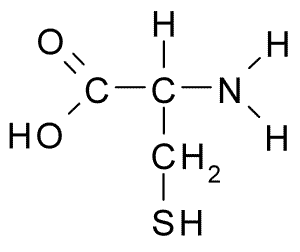
\includegraphics[width=0.8\linewidth]{secProteins/figures/cysteine.png}	
			\caption{Cisteína}
			\label{fig:cysteine}
		\end{minipage}
		\begin{minipage}{0.3\linewidth}
			\centering   
			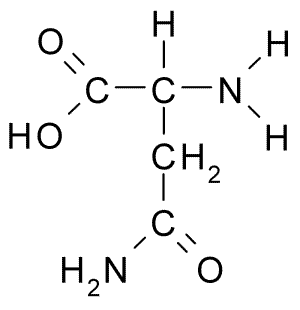
\includegraphics[width=0.65\linewidth]{secProteins/figures/asparagine.png}
			\caption{Asparagina}
			\label{fig:asparagine}
		\end{minipage}
		\begin{minipage}{0.3\linewidth}
			\centering   
			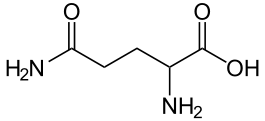
\includegraphics[width=1\linewidth]{secProteins/figures/glutamine.png}
			\caption{Glutamina}
			\label{fig:glutamine}
		\end{minipage}
	\end{center}
\end{figure}
\vspace{-1cm}
\begin{figure}[H]
	\begin{center}
		\begin{minipage}{0.45\linewidth}
			\centering   
			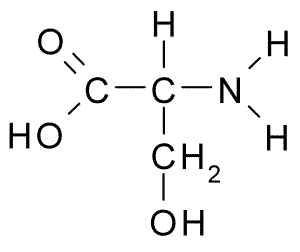
\includegraphics[width=0.5\linewidth]{secProteins/figures/serine.png}	
			\caption{Serina}
			\label{fig:serine}
		\end{minipage}
		\begin{minipage}{0.45\linewidth}
			\centering   
			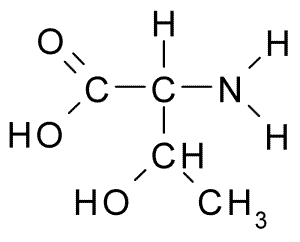
\includegraphics[width=0.5\linewidth]{secProteins/figures/threonine.png}
			\caption{Treonina}
			\label{fig:threonine}
		\end{minipage}
	\end{center}
\end{figure}

\subsubsection*{Grupos R aromáticos}
\begin{figure}[H]
	\begin{center}
		\begin{minipage}{0.3\linewidth}
			\centering   
			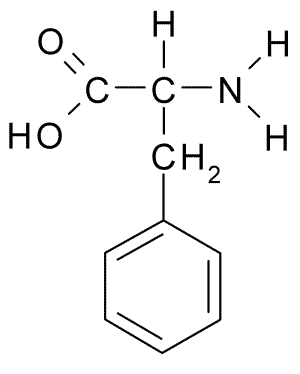
\includegraphics[width=0.7\linewidth]{secProteins/figures/phenylalanine.png}	
			\caption{Fenilalanina}
			\label{fig:phenylalanine}
		\end{minipage}
		\begin{minipage}{0.3\linewidth}
			\centering   
			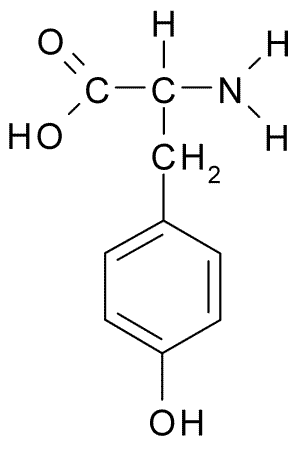
\includegraphics[width=0.59\linewidth]{secProteins/figures/tyrosine.png}
			\caption{Tirosina}
			\label{fig:tyrosine}
		\end{minipage}
		\begin{minipage}{0.3\linewidth}
			\centering   
			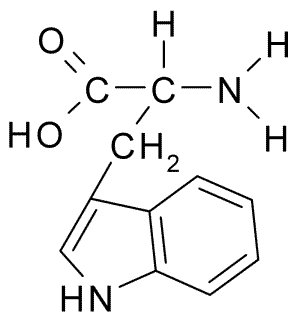
\includegraphics[width=0.7\linewidth]{secProteins/figures/tryptophan.png}
			\caption{Triptofano}
			\label{fig:tryptophan}
		\end{minipage}
	\end{center}
\end{figure}

\subsubsection*{Grupos R carregados positivamente}
\begin{figure}[H]
	\begin{center}
		\begin{minipage}{0.3\linewidth}
			\centering   
			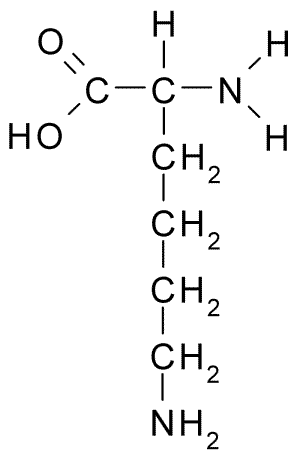
\includegraphics[width=0.7\linewidth]{secProteins/figures/lysine.png}	
			\caption{Lisina}
			\label{fig:lysine}
		\end{minipage}
		\begin{minipage}{0.3\linewidth}
			\centering   
			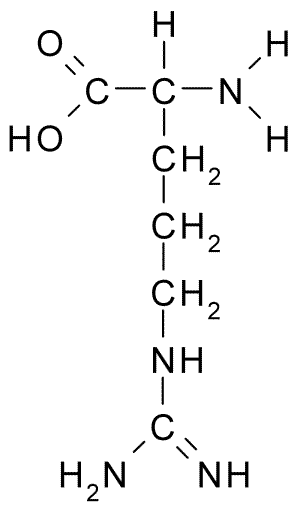
\includegraphics[width=0.59\linewidth]{secProteins/figures/arginine.png}
			\caption{Arginina}
			\label{fig:arginine}
		\end{minipage}
		\begin{minipage}{0.3\linewidth}
			\centering   
			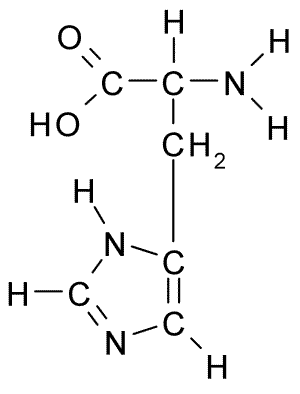
\includegraphics[width=0.7\linewidth]{secProteins/figures/histidine.png}
			\caption{Histidina}
			\label{fig:histidine}
		\end{minipage}
	\end{center}
\end{figure}

\subsubsection*{Grupos R carregados negativamente}

\begin{figure}[H]
	\begin{center}
		\begin{minipage}{0.45\linewidth}
			\centering   
			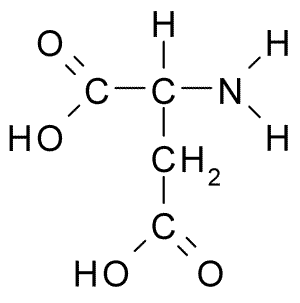
\includegraphics[width=0.5\linewidth]{secProteins/figures/asparticacid.png}	
			\caption{Aspartato}
			\label{fig:asparticacid}
		\end{minipage}
		\begin{minipage}{0.45\linewidth}
			\centering   
			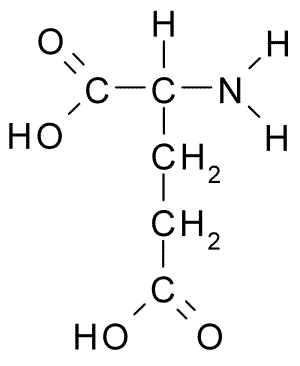
\includegraphics[width=0.45\linewidth]{secProteins/figures/glutamicacid.png}
			\caption{Glutamato}
			\label{fig:glutamicacid}
		\end{minipage}
	\end{center}
\end{figure}
